\documentclass[../main.tex]{subfiles}
\begin{document}

The plan is to show all finitely generated reflection groups are in fact Coxeter groups, which admit a nice geometric classification. This follows\cite{Humphreys1990}

This is a rough outline of the structure:

\subsection{Reflection groups}

work in $n$-dimensional euclidean space $E$.

consider the group of affine transformations $GL(E)\ltimes E$, with inner product preserving subgroup $O$.

A reflection in $E$ is an affine transformation $r\in O$ that  fixes some affine hyperplane $H$ (linear transformation of codimension $1$ subspace).

a reflection group $W$ is generated by reflections in the euclidean space. let $\cH$ by the set of hyperplanes $H_i\subseteq E$ fixed by some reflection $r_i\in W$. 

Choosing a unit normal vector $\alpha_i$ to each $H_i$ gives a \textbf{root system} $\Phi$. 

We can derive the Coxeter relations from $\Phi$, a group satisfying such relations is called Coxeter.

\begin{definition}
    We call a group $W$ \textbf{Coxeter} if it admits a presentation of the form:\[
    \abr{r_1,\ldots,r_n \mid (r_ir_j)^{m_{ij}}\text{ for all }i,j}
    \]
    where each $m_{ij}\in \bN\cup\{\infty\}$, and $m_{ii}=1$ for all $i$. For formal reasons, we will consider the pair $(W,R)$, where $R$ is the set of generators in the presentation, and call this a \textbf{Coxeter system}. We call a Coxeter system finite if $R$ is finite.
\end{definition}

\subsection{The fundamental domain}

The action of $W$ fixes $\Phi$ and $\cH$ so acts on the connexted componenets $E\setminus\cH$ called the set of \textbf{fundamental domains} for $W$. 

The reflections fixing hyperplanes bounding any single fundamental domain will generate $W$, such reflections (hyperplanes, roots) are called \textbf{simple}.

Show the action of $W$ on the fundamental domains is transitive

\subsection{Words}

The length of a word in terms of simple reflections corresponds to the number of plane between a fundamental domain and its image. This implies the action on fundamental domains is in fact \textbf{simply} transitive.

\begin{proposition}[Deletion condition]
    Given an unreduced expression $w=r_1\cdots r_k$ there exists $1\leq i < j \leq k$ such that $w=r_1\cdots\hat{r_i}\cdots\hat{r_j}\cdots r_k$, where the hat means ommitance.
\end{proposition}

\begin{proposition}[Exchange condition]
    For $w=r_1\cdots r_k$ a not necessarily reduced expression and some simple $r\in W$ with $l(wr)<l(w)$, then there exists an $1\leq i\leq k$ s.t. $wr = r_1\cdots\hat{r_i}\cdots r_k$.
\end{proposition}

\begin{theorem}
    Any non-trivial relation in a reflection group is a consequence of the Coxeter relations.
\end{theorem}

\subsection{Classification}

To any finite Coxeter system $(W,R)$ we can associate an undirected graph called its \textbf{Coxeter diagram} by the following rules:\begin{itemize}
    \item Draw a node $i$ for each $r_i\in R$;
    \item For each relation $(r_i r_j)^{m_{ij}}$ with $m_{ij}>2$ draw an edge between $i$ and $j$ and label it with $m_{ij}$.
\end{itemize}

This process can be reversed to obtain a Coxeter system from any Coxeter diagram. This correspondence will associate the graph:
\begin{figure}[!h]
\centering
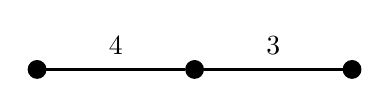
\begin{tikzpicture}
    \begin{scope}[every node/.style={circle, fill=black, draw, thick, minimum size = 6pt, inner sep=0pt}]
        \node (1) at (0,0) {};
        \node (2) at (2,0) {};
        \node (3) at (4,0) {};
    \end{scope}

    \begin{scope}[every edge/.style={draw,very thick}]
        \path [-] (1) edge (2);
        \path [-] (2) edge (3);
        \node at (1,0.3) {$4$};
        \node at (3,0.3) {$3$};
    \end{scope}
\end{tikzpicture}
\end{figure}

to the group presentation: \[
\abr{r_1,r_2,r_3 \ \middle| \ r_1^2 = r_2^2 = r_3^2 = e, \ (r_1r_2)^4 = (r_2r_3)^3 = (r_1r_3)^2 = e}
\]

For brevity the $3$ labels will often  be excluded.

\begin{itemize}
    \item show the graph is well defined up isometryish
    \item disjoint unions of graphs correspond to products of groups
    \item bilinear form of a coxeter group
    \item if positive define the coxeter group is finite
    \item classify positive-definite forms
    \item all of which can be seen as reflection groups of regular polyhedra. some of which will be described in the previous section?
\end{itemize}

\begin{figure}[!h]
\resizebox{\textwidth}{!}{
\begin{tikzpicture}
    \begin{scope}[shift={(0,0)}]
        \node at (0,0) {$A_n$};
        \begin{scope}[every node/.style={circle, fill=black, draw, thick, minimum size = 6pt, inner sep=0pt}]
            \node (1) at (2,0) {};
            \node (2) at (4,0) {};
            \node (3) at (6,0) {};
            \node (n-2) at (10,0) {};
            \node (n-1) at (12,0) {};
            \node (n) at (14,0) {};
        \end{scope}
        \node (3a) at (7,0) {};
        \node (3b) at (9,0) {};
        \begin{scope}[every edge/.style={draw,very thick}]
            \path [-] (1) edge (2);
            \path [-] (2) edge (3a);
            \path [loosely dashed] (3a.west) edge (3b.east);
            \path [-] (3b) edge (n-1);
            \path [-] (n-1) edge (n);
        \end{scope}
        \node at (16,0) {$(n\geq 1)$};
    \end{scope}

    \begin{scope}[shift={(0,-1.5)}]
        \node at (0,0) {$BC_n$};
        \begin{scope}[every node/.style={circle, fill=black, draw, thick, minimum size = 6pt, inner sep=0pt}]
            \node (1) at (2,0) {};
            \node (2) at (4,0) {};
            \node (3) at (6,0) {};
            \node (n-2) at (10,0) {};
            \node (n-1) at (12,0) {};
            \node (n) at (14,0) {};
        \end{scope}
        \node (3a) at (7,0) {};
        \node (3b) at (9,0) {};
        \begin{scope}[every edge/.style={draw,very thick}]
            \path [-] (1) edge (2);
            \path [-] (2) edge (3a);
            \path [loosely dashed] (3a.west) edge (3b.east);
            \path [-] (3b) edge (n-1);
            \path [-] (n-1) edge (n);
            \node at (13,0.3) {$4$};
        \end{scope}
        \node at (16,0) {$(n\geq 2)$};
    \end{scope}

    \begin{scope}[shift={(0,-5)}]
        \node at (0,0) {$D_n$};
        \begin{scope}[every node/.style={circle, fill=black, draw, thick, minimum size = 6pt, inner sep=0pt}]
            \node (1) at (2,0) {};
            \node (2) at (4,0) {};
            \node (3) at (6,0) {};
            \node (n-2) at (10,0) {};
            \node (n-1) at (12,0) {};
            \node (n-1a) at (12,2) {};
            \node (n) at (14,0) {};
        \end{scope}
        \node (3a) at (7,0) {};
        \node (3b) at (9,0) {};
        \begin{scope}[every edge/.style={draw,very thick}]
            \path [-] (1) edge (2);
            \path [-] (2) edge (3a);
            \path [loosely dashed] (3a.west) edge (3b.east);
            \path [-] (3b) edge (n-1);
            \path [-] (n-1) edge (n-1a);
            \path [-] (n-1) edge (n);
        \end{scope}
        \node at (16,0) {$(n\geq 4)$};
    \end{scope}

    \begin{scope}[shift={(0,-8.5)}]
        \node at (0,0) {$E_6$};
        \begin{scope}[every node/.style={circle, fill=black, draw, thick, minimum size = 6pt, inner sep=0pt}]
            \node (1) at (2,0) {};
            \node (2) at (4,0) {};
            \node (3) at (6,0) {};
            \node (4) at (6,2) {};
            \node (5) at (8,0) {};
            \node (6) at (10,0) {};
        \end{scope}
        \begin{scope}[every edge/.style={draw,very thick}]
            \path [-] (1) edge (2);
            \path [-] (2) edge (3);
            \path [-] (3) edge (4);
            \path [-] (3) edge (5);
            \path [-] (5) edge (6);
        \end{scope}
    \end{scope}

    \begin{scope}[shift={(0,-12)}]
        \node at (0,0) {$E_7$};
        \begin{scope}[every node/.style={circle, fill=black, draw, thick, minimum size = 6pt, inner sep=0pt}]
            \node (1) at (2,0) {};
            \node (2) at (4,0) {};
            \node (3) at (6,0) {};
            \node (4) at (8,0) {};
            \node (5) at (8,2) {};
            \node (6) at (10,0) {};
            \node (7) at (12,0) {};
        \end{scope}
        \begin{scope}[every edge/.style={draw,very thick}]
            \path [-] (1) edge (2);
            \path [-] (2) edge (3);
            \path [-] (3) edge (4);
            \path [-] (4) edge (5);
            \path [-] (4) edge (6);
            \path [-] (6) edge (7);
        \end{scope}
    \end{scope}

    \begin{scope}[shift={(0,-15.5)}]
        \node at (0,0) {$E_8$};
        \begin{scope}[every node/.style={circle, fill=black, draw, thick, minimum size = 6pt, inner sep=0pt}]
            \node (1) at (2,0) {};
            \node (2) at (4,0) {};
            \node (3) at (6,0) {};
            \node (4) at (8,0) {};
            \node (5) at (10,0) {};
            \node (6) at (10,2) {};
            \node (7) at (12,0) {};
            \node (8) at (14,0) {};
        \end{scope}
        \begin{scope}[every edge/.style={draw,very thick}]
            \path [-] (1) edge (2);
            \path [-] (2) edge (3);
            \path [-] (3) edge (4);
            \path [-] (4) edge (5);
            \path [-] (5) edge (6);
            \path [-] (5) edge (7);
            \path [-] (7) edge (8);
        \end{scope}
    \end{scope}

    \begin{scope}[shift={(0,-17)}]
        \node at (0,0) {$F_4$};
        \begin{scope}[every node/.style={circle, fill=black, draw, thick, minimum size = 6pt, inner sep=0pt}]
            \node (1) at (2,0) {};
            \node (2) at (4,0) {};
            \node (3) at (6,0) {};
            \node (4) at (8,0) {};
        \end{scope}
        \begin{scope}[every edge/.style={draw,very thick}]
            \path [-] (1) edge (2);
            \path [-] (2) edge (3);
            \path [-] (3) edge (4);
            \node at (5,0.3) {$4$};
        \end{scope}
    \end{scope}

    \begin{scope}[shift={(0,-18.5)}]
        \node at (0,0) {$H_3$};
        \begin{scope}[every node/.style={circle, fill=black, draw, thick, minimum size = 6pt, inner sep=0pt}]
            \node (1) at (2,0) {};
            \node (2) at (4,0) {};
            \node (3) at (6,0) {};
        \end{scope}
        \begin{scope}[every edge/.style={draw,very thick}]
            \path [-] (1) edge (2);
            \path [-] (2) edge (3);
            \node at (3,0.3) {$5$};
        \end{scope}
    \end{scope}

    \begin{scope}[shift={(0,-20)}]
        \node at (0,0) {$H_4$};
        \begin{scope}[every node/.style={circle, fill=black, draw, thick, minimum size = 6pt, inner sep=0pt}]
            \node (1) at (2,0) {};
            \node (2) at (4,0) {};
            \node (3) at (6,0) {};
            \node (4) at (8,0) {};
        \end{scope}
        \begin{scope}[every edge/.style={draw,very thick}]
            \path [-] (1) edge (2);
            \path [-] (2) edge (3);
            \path [-] (3) edge (4);
            \node at (3,0.3) {$5$};
        \end{scope}
    \end{scope}

    \begin{scope}[shift={(0,-21.5)}]
        \node at (0,0) {$I_2(m)$};
        \begin{scope}[every node/.style={circle, fill=black, draw, thick, minimum size = 6pt, inner sep=0pt}]
            \node (1) at (2,0) {};
            \node (2) at (4,0) {};
        \end{scope}
        \begin{scope}[every edge/.style={draw,very thick}]
            \path [-] (1) edge (2);
            \node at (3,0.3) {$m$};
            \node at (6,0) {$(m\geq 4)$};
        \end{scope}
    \end{scope}
\end{tikzpicture}
}
\end{figure}

\end{document}